\documentclass[11pt]{article}
\usepackage[margin=1in]{geometry}
\usepackage[T1]{fontenc}
\usepackage{lmodern}
\usepackage{amsmath,amssymb}
\usepackage{booktabs,tabularx}
\usepackage{enumitem}
\usepackage{xcolor}
\usepackage{tikz}
\usetikzlibrary{positioning,arrows.meta}
\usepackage[hidelinks]{hyperref}
\usepackage[numbers,sort]{natbib}

% Notes to yourself while editing. Make \note print nothing once the handout is done:
%   \renewcommand{\note}[1]{}
\newcommand{\note}[1]{\textcolor{orange!80!black}{\small[\textbf{Edit:} #1]}}
\newcommand{\verify}{\textcolor{red!70!black}{\small[verify]}}
\newcommand{\proves}{\vdash}

\title{Legal Moves and Book Knowledge:\\
\large Can LLMs Build Textbook Deductions that Lean Accepts?}
\author{Research plan \note{your name}}
\date{Draft, November 2026}

\begin{document}
\maketitle

\begin{abstract}
\noindent
Large language models write proofs that look right and fail when checked. This project asks whether two kinds of structure make them more reliable on formal deductions in propositional logic. The first is \emph{knowing which moves are legal}, encoded in PDDL. The second is \emph{knowing what the textbook says}, encoded as a knowledge graph. The setting is the deduction system of Mileti's \emph{A Mathematical Introduction to Mathematical Logic}~\cite{mileti2020}, Chapters~1--3. At each step an LLM chooses one of Mileti's fourteen rules. Code I write by hand in Lean~4 checks the step, which acts as a ``gate''. I compare the LLM alone, the LLM with legal moves, and the LLM with legal moves plus the knowledge graph, on a small and a large model. The main outputs are success rates and a taxonomy of where models fail.
\end{abstract}

\section{Motivation}
\begin{itemize}[leftmargin=*]
  \item LLMs plan and prove badly on their own, but do well when paired with an external checker~\cite{kambhampati2024llmmodulo,valmeekam2023planbench}. In theorem proving, the checker is a proof assistant~\cite{yang2023leandojo,thakur2024copra}.
  \item Most LLM theorem-proving work targets competition maths in Mathlib. Logic textbooks are a cleaner test: the rules are few, explicit and fully mechanical.
  \item \emph{Proof planning}~\cite{bundy1988,bundy1996proofplanning} treated proof search as planning: a planner chooses high-level methods whose preconditions are checked. This project revives that idea. The planner becomes an LLM, the preconditions are PDDL~\cite{mcdermott1998pddl}, and the checker is Lean.
  \item This continues my earlier work: a procedural knowledge graph for a small calculus-solving LLM (graded by SymPy), and a knowledge-graph-plus-Lean pipeline for philosophy. \note{1--2 sentences with your actual results, e.g.\ 26/30 right method, oracle 6/10 vs graph 4/10.}
\end{itemize}

\section{Research questions}
\begin{description}[leftmargin=*,font=\normalfont\bfseries]
  \item[RQ1 (legal moves).] Does telling the LLM which rules are legal at each step raise the share of deductions Lean accepts and lower the number of rejected steps?
  \item[RQ2 (book knowledge).] Does a knowledge graph of the textbook (definitions, rules, worked examples, strategies, pitfalls) help beyond legal moves? Does a hand-written graph beat an LLM-extracted one?
  \item[RQ3 (model size).] Do these effects differ between a small and a large model? Recent work reports that graph context helps small provers but can hurt large ones~\cite{nabi2026structured}.
  \item[RQ4 (failures).] Where do LLMs fail in Mileti's system? Candidate categories: wrong rule shape, assumption-order errors with $\to$I, missing a proof by contradiction, and unhelpful choices of free formulas.
\end{description}
\note{Add or cut RQs. Write down your predicted answer to each before running anything.}

\section{The proof system (Mileti \S3.4)}
A \emph{line} is a pair $S \proves \varphi$, where $S$ is a finite \emph{sequence} of formulas (order and repeats matter). A \emph{deduction} is a sequence of lines. Each line is an assumption or follows from earlier lines by a rule.

\medskip
\begin{center}
\small
\begin{tabular}{@{}lll@{}}
\toprule
Rule & From & Conclude \\
\midrule
Assume & --- & $S \proves \varphi$ \quad ($\varphi$ in $S$) \\
$\wedge$EL / $\wedge$ER & $S \proves \varphi\wedge\psi$ & $S\proves\varphi$ \ / \ $S\proves\psi$ \\
$\wedge$I & $S\proves\varphi$,\ $S\proves\psi$ & $S\proves\varphi\wedge\psi$ \\
$\vee$IL / $\vee$IR & $S\proves\varphi$ \ / \ $S\proves\psi$ & $S\proves\varphi\vee\psi$ \\
$\to$E & $S\proves\varphi\to\psi$ & $S,\varphi\proves\psi$ \\
$\to$I & $S,\varphi\proves\psi$ & $S\proves\varphi\to\psi$ \\
$\vee$PC & $S,\varphi\proves\theta$,\ $S,\psi\proves\theta$ & $S,\varphi\vee\psi\proves\theta$ \\
$\neg$PC & $S,\psi\proves\varphi$,\ $S,\neg\psi\proves\varphi$ & $S\proves\varphi$ \\
Contr & $S,\neg\varphi\proves\psi$,\ $S,\neg\varphi\proves\neg\psi$ & $S\proves\varphi$ \\
Expand / Delete & $S\proves\varphi$ \ / \ $S,\gamma,\gamma\proves\varphi$ & $S,\gamma\proves\varphi$ \\
Reorder & $S_1,\gamma_1,\gamma_2,S_2\proves\varphi$ & $S_1,\gamma_2,\gamma_1,S_2\proves\varphi$ \\
\bottomrule
\end{tabular}
\end{center}

\section{System}
\begin{center}
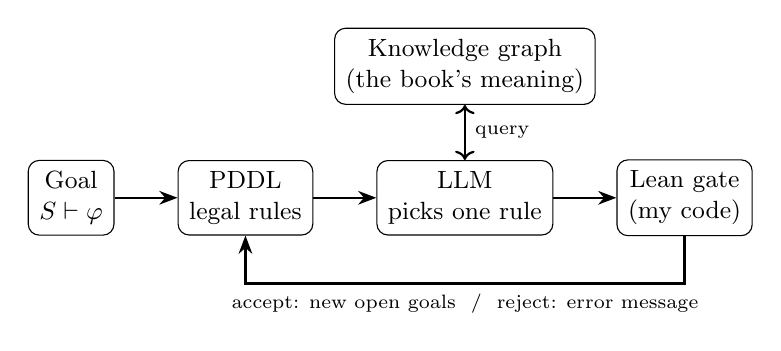
\begin{tikzpicture}[
  box/.style={draw,rounded corners,align=center,minimum height=9mm,inner sep=4pt,font=\small},
  arr/.style={-{Stealth},thick}]
  \node[box] (goal) {Goal\\$S\proves\varphi$};
  \node[box,right=8mm of goal] (pddl) {PDDL\\legal rules};
  \node[box,right=8mm of pddl] (llm) {LLM\\picks one rule};
  \node[box,right=8mm of llm] (lean) {Lean gate\\(my code)};
  \node[box,above=7mm of llm] (kg) {Knowledge graph\\(the book's meaning)};
  \draw[arr] (goal) -- (pddl);
  \draw[arr] (pddl) -- (llm);
  \draw[arr] (llm) -- (lean);
  \draw[arr,<->] (kg) -- node[right,font=\scriptsize]{query} (llm);
  \draw[arr] (lean.south) -- ++(0,-6mm) -| node[pos=0.25,below,font=\scriptsize]{accept: new open goals \ / \ reject: error message} (pddl.south);
\end{tikzpicture}
\end{center}

\begin{enumerate}[leftmargin=*]
  \item \textbf{Lean gate (written by me).} An inductive \texttt{Formula}; a predicate \texttt{Derivable : List Formula $\to$ Formula $\to$ Prop} with one constructor per rule, mirroring Mileti's definition of deductions as a generating system; and a computable step checker that reports which side condition failed. Stretch goal: prove soundness (\S3.5) in Lean.
  \item \textbf{PDDL domain (written by me).} One action per rule. Search runs backward from the goal: an action closes one open goal and opens its premises. Four rules need a formula the goal does not contain ($\wedge$EL, $\wedge$ER, $\neg$PC, Contr). For these, arguments come from a finite candidate set: subformulas of the goal and assumptions, closed under one negation.
  \item \textbf{Knowledge graph (written by me).} Nodes are definitions, rules, worked examples, strategies, pitfalls and theorems. Edges are \texttt{depends\_on}, \texttt{uses\_rule}, \texttt{illustrates}, \texttt{strategy\_for} and \texttt{pitfall\_of}. Everything is in my own words, with section references. A second graph is extracted by an LLM pipeline, as a comparison.
  \item \textbf{LLM loop.} At each step the LLM sees the open goals and (by condition) the legal moves, and may query the graph. It outputs one rule application. Lean accepts or rejects it, and errors go back to the LLM. The loop stops at a proof or when the step budget runs out.
\end{enumerate}

\section{Benchmark}
Chapters 2--3 contain only nine object-level deductions: six in \S3.4 and Exercises~3.7.7, 3.7.8(a) and 3.7.8(b). The rest are proofs \emph{about} the system or about truth tables. So:
\begin{itemize}[leftmargin=*]
  \item \textbf{Book set (9):} a development and sanity check.
  \item \textbf{Generated set (100--200):} random sequents over 2--4 atoms. Each is kept only if valid by truth table; by completeness (\S3.5), every valid sequent has a deduction. Difficulty is the length of the shortest proof found by a planner~\cite{helmert2006fastdownward}. Fresh items avoid training-data contamination.
\end{itemize}

\section{Experiment}
\begin{center}
\small
\begin{tabularx}{\linewidth}{@{}lX@{}}
\toprule
Condition & What the LLM gets \\
\midrule
A.\ LLM alone & Goal, rule list, Lean feedback \\
B.\ + PDDL & A, plus the legal moves at each step \\
C.\ + PDDL + KG & B, plus queries to the hand-written graph \\
D.\ + PDDL + extracted KG & B, plus the LLM-built graph \\
E.\ Oracle & B, plus the correct strategy up front \\
\bottomrule
\end{tabularx}
\end{center}
Models: one small open model and one strong API model, 3+ seeds each, with a fixed step budget. \note{Name the models.}\\
Metrics: proofs accepted (\%), steps per proof, rejected steps, proposals outside the candidate set, and the failure taxonomy. Conditions are compared with paired McNemar tests.

\section{Related work and how this differs}
\begin{description}[leftmargin=*,font=\normalfont\bfseries]
  \item[LLMs and natural deduction.] ProofGrid~\cite{arkoudas2025stress} tests LLMs on writing and checking proofs in a minimal natural-deduction language, with mechanical grading. Its authors find that hard tasks remain unsolved. \emph{Difference:} I build proofs one step at a time with legal-move constraints and textbook knowledge, and measure what each layer adds. Related: trial-and-error fine-tuning for intuitionistic propositional logic in Lean~\cite{an2024learn}.
  \item[LLMs and planning.] LLM+P~\cite{liu2023llmp} hands planning to a classical planner. LLM-Modulo~\cite{kambhampati2024llmmodulo} and PlanBench~\cite{valmeekam2023planbench} argue that LLMs need external verifiers. \emph{Difference:} PDDL here constrains the LLM's moves rather than replacing the LLM.
  \item[LLM theorem proving in Lean.] GPT-f~\cite{polu2020gptf}, LeanDojo/ReProver~\cite{yang2023leandojo}, LLMSTEP~\cite{welleck2023llmstep}, COPRA~\cite{thakur2024copra}, DeepSeek-Prover-V2~\cite{ren2025deepseekproverv2}. These target Mathlib and competition maths, not a fixed textbook proof system.
  \item[Knowledge graphs for proving.] MathKG~\cite{nabi2026structured} and ProofWiki-graph agents~\cite{proofwikikg2025}. \emph{Difference:} a small, hand-written graph of one textbook, compared directly with an extracted one.
  \item[Proof planning.] Bundy's proof plans and rippling~\cite{bundy1988,bundy1996proofplanning,bundy2005rippling}. Planning as theorem proving~\cite{green1969}.
  \item[Formalized propositional logic.] Isabelle~\cite{michaelis2018formalized}, Coq~\cite{vandoorn2015coq}, Lean (intuitionistic)~\cite{trufas2024ipl}. These are references for my own Lean code.
\end{description}
\note{After reading each paper, add one line on what you take from it.}

\section{Timeline}
\begin{center}
\small
\begin{tabularx}{\linewidth}{@{}lX@{}}
\toprule
When & Milestone \\
\midrule
Nov--Dec 2026 & \texttt{Formula} and all 14 rules in Lean; the 9 book deductions proved; graph v0 ($\sim$30 nodes) \\
Jan 2027 & Independent study begins \note{supervisor} \\
Feb--Mar 2027 & PDDL domain, loop, generated benchmark; all conditions with one model \\
Apr--May 2027 & Second model, seeds, failure taxonomy; draft paper \\
Summer 2027 & Workshop submission (AI for Math / MATH-AI / NeSy); arXiv \\
\bottomrule
\end{tabularx}
\end{center}

\section{Reading list, in priority order}
\begin{enumerate}[leftmargin=*]
  \item Arkoudas \& Batzoglou~\cite{arkoudas2025stress}, the closest prior work. Read first and sharpen the ``difference'' above.
  \item Nabi et al.~\cite{nabi2026structured}: when graph context helps or hurts (RQ2--3).
  \item Kambhampati et al.~\cite{kambhampati2024llmmodulo}: the LLM plus external checker framing.
  \item Bundy~\cite{bundy1996proofplanning}: proof planning, the historical root.
  \item Thakur et al.~\cite{thakur2024copra}: an in-context LLM agent with prover feedback, close to my loop.
  \item Yang et al.~\cite{yang2023leandojo}: the standard LLM plus Lean setup.
  \item Michaelis \& Nipkow~\cite{michaelis2018formalized}: how others formalized these proof systems.
  \item Liu et al.~\cite{liu2023llmp}, Valmeekam et al.~\cite{valmeekam2023planbench}: LLMs and PDDL.
\end{enumerate}

\section{Open questions}
\begin{itemize}[leftmargin=*]
  \item Should PDDL track assumption \emph{order} with position facts, or leave sequences to the Python checker?
  \item Should the LLM output Lean syntax directly, or a structured rule call that Python translates?
  \item Which supervisor and co-advisor? \note{fill in}
\end{itemize}

\bibliographystyle{plainnat}
\bibliography{refs}
\end{document}
